\section{Probabilistic Input  Markov Chain}
\label{sec:pmac}
\subsection{Developing on independent Markov chains}
The IMAC method considers an observation to be either occupied or free. In the system setup used in this project, however, the input is the probability that a cell is occupied. To use IMAC it is necessary to determine the state of the observation with one or two thresholds. The simplest choice is placing a threshold at $0.5$ rendering everything above as an occupied observation and everything below a free. This approach will make no distinction between an observation of $0.501$ and $0.999$, which both will be considered occupied and contribute equally in the learning process. This is not desirable as the latter measurement contains immensely more information than the former. 
Equating all measurements on the basis that they fall on the same side of a threshold reduces the advantage of taking position and sensor noise into consideration. An example could be a cell observed at a great distance and quite large uncertainty and then later very close by with high confidence in the reading. These two entries into the IMAC learner would carry the same weight. If for instance a reading resulted in a $0.99$ occupancy probability and a following reading produced a $0.49$ occupancy probability, the simple threshold method would register it as an occupied followed by a free and thus adding an event. In reality there is very little evidence for this event happening and if the subsequent reading would again produce a $0.99$ occupancy probability this would introduce even more dynamics disregarding that the evidence is very unsubstantiated. 

Therefore a method of incorporating the uncertainty of the observations and carrying them into the learner is desired. As IMAC is a fast learner of Markov transition probabilities when the observations are very certain, the incorporation of the uncertainties should not hinder that. 

The requirements for the incorporation of the uncertainties are:
\begin{itemize}
	\item Perform as IMAC on perfect input
	\item Avoid low confidence observations counting as much as high confidence
	\item Avoid biasing towards neither static or dynamic
\end{itemize}

The method devised to accomplish the integration of uncertainties is denoted probability input Markov chain (PMAC). As opposed to IMAC the PMAC uses a score rather than a count of a state and event. The state score is calculated as  \(2\cdot|0.5-p_{occ}|\) for the active state which is determined by whether \(p_{occ} > 0.5\) or not. This ensures that if the reading is certain, ie. either 0 or 1 the update will be similar to that of IMAC, and as uncertainty increases the score linearly decreases. The event score is calculated based on how certain the previous state was and how certain the current state is. In order to avoid biasing towards dynamic the maximum, based on the certainty of the previous state, is the average of the consecutive observations in that state. As the average cannot exceed 1 this ensures that in perfect certainty the behavior is equal to that of IMAC. The maximum limit based on the current state is the sum of scores in the current state.

\begin{equation}
IMAC: \lambda = \frac{\#event_{count}}{\#state_{obs}}
\end{equation}

\begin{equation}
PMAC: \lambda = \frac{\Sigma event_{score}}{\Sigma state_{score}}
\end{equation}

\begin{equation}
state_{score}=2 \cdot |0.5-p_{occ}| 
\end{equation}

\begin{equation}
event_{score}=min(\hat{\mu}_{state_{score}}(i-1),state_{score}(i))
\end{equation}

Both the state and event scores behave as IMAC counters when the certainty is perfect, thus fulfilling the first requirement. The second requirement is achieved by the state score scaling with the occupancy probability distance from $0.5$, and the event score basing its value on the state score. Basing the state score on the distance from $0.5$ helps to avoid skewing the result towards static. Another possible scoring could be the probability for occupied and free respectively: 

\begin{equation}
score_{occ} = p_{occ}
\end{equation}
\begin{equation}
score_{free} = 1-p_{occ}
\end{equation}

As the active state is determined by a threshold of $0.5$, this scoring system would always be at least $0.5$, skewing the results. The chosen score better incorporates $0.5$ denoting unknown, thus producing a score of $0$. 

In order to avoid biasing towards dynamic the average of the previous state scores is used. If, instead, the sum had been used, a series of low confidence observations could skew the result. As the state score can be considered $\hat{\mu} \cdot n_{obs}$ the event score will be balanced when using as a maximum value. For instance $5$ observation with an occupancy probability of $0.6$ would each give a score of $0.2$, and the sum would consequently be $1$. Using the sum,  would be $1/1$  thus skewing it towards dynamics. Using the average, the event score is balanced to the state score and produces a more correct value of $0.2/1$. The correctness of this result is evident from the fact that simply counting events and states with IMAC also results in a probability on $\lambda = 1/5$. Hence the correct dynamics is estimated with PMAC and the parameters are only updated according to the confidence in the used observations.

\subsection{PMAC in action - an example}
Figure \ref{fig:state_scores_explained} shows an example of some observation, their occupied probabilities $p_{occ}$ and the subsequent state score. On the score plot the average of sequential observation in the same state are shown as green lines. This sets a maximum limit on the size of the subsequent event score. To demonstrate the workings of PMAC these observations are used as input to the PMAC learner in the following. 

\begin{figure} [htbp]
    \centering
    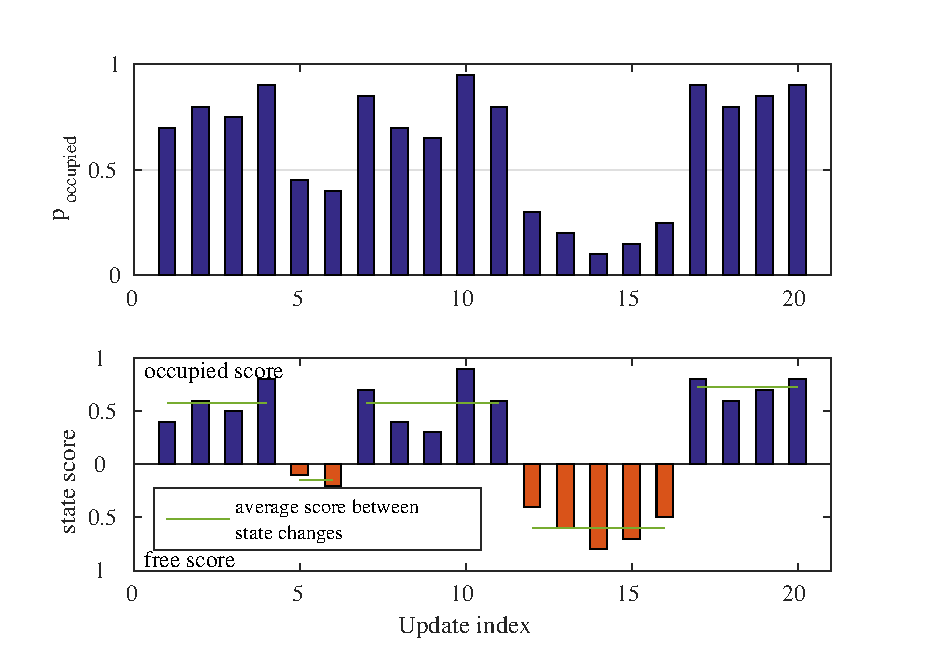
\includegraphics[scale=1]{chapters/mapping_of_dynamic_areas/figures/state_scores_explained}
    \caption{Artificial example of occupancy probabilities used to learn dynamics.}
    \label{fig:state_scores_explained}
\end{figure}

From the state scores in figure \ref{fig:state_scores_explained} it is seen that from index 0 to 11, the situation starts as occupied with quite confident readings. Then $2$ more uncertain reading showing free occurs before confident readings of occupied are again received. The effect of this on the exit is shown in figure \ref{fig:pmac_exit_explained}. The sum of occupied scores increases steadily from index $0$ to $11$, while the event sum increases a comparatively small amount. However it is clearly visible on the exit  value as it is the first observations and both sums are initialized to the smallest possible non-zero value. This initialization is chosen in order to avoid dividing by $0$ and minimizing the effect of the initialization on the result. The effects of this initialization is clearly visible in figure \ref{fig:pmac_entry_explained}, that shows the scores and values for the entry. The entry value is $1$, as the initial values causes, but as soon as input is received their effect is suppressed.

\begin{figure}[htbp]
\centering
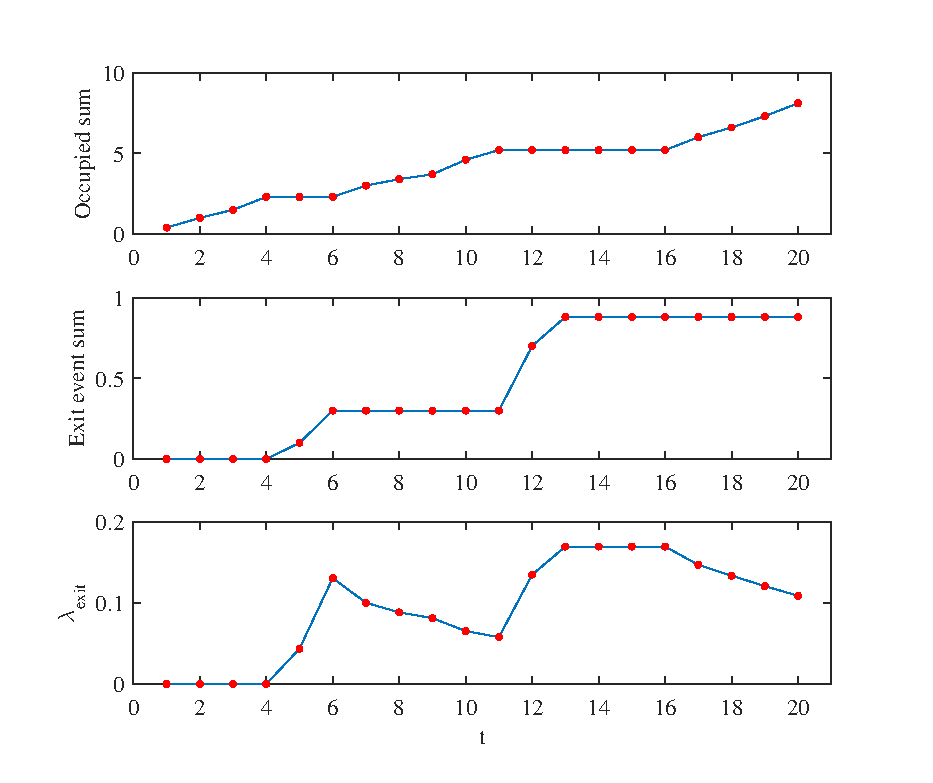
\includegraphics[scale=1]{chapters/mapping_of_dynamic_areas/figures/pmac_exit_explained}
\caption{Evolution of parameters used to estimate dynamics with the data shown in figure \ref{fig:state_scores_explained}.}
\label{fig:pmac_exit_explained}
\end{figure}

The observations from index $7$ to $20$ constitutes more certain changes in the state and thus carry more information which can be seen in the sums of especially the free score and entry event score. 

\begin{figure}[htbp]
    \centering
    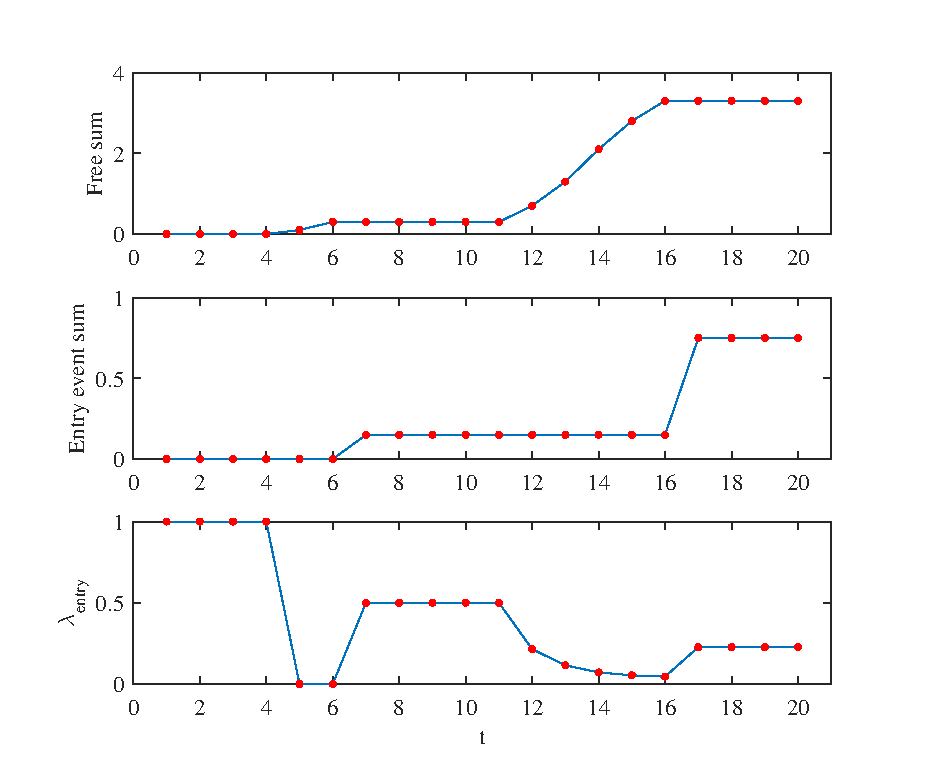
\includegraphics[scale=1]{chapters/mapping_of_dynamic_areas/figures/pmac_entry_explained}
    \caption{Evolution of parameters used to estimate dynamics with the data shown in figure \ref{fig:state_scores_explained}.}
    \label{fig:pmac_entry_explained}
\end{figure}

\todo{Write about improved pmac handling noise problem}

\begin{figure}[htbp]
\centering
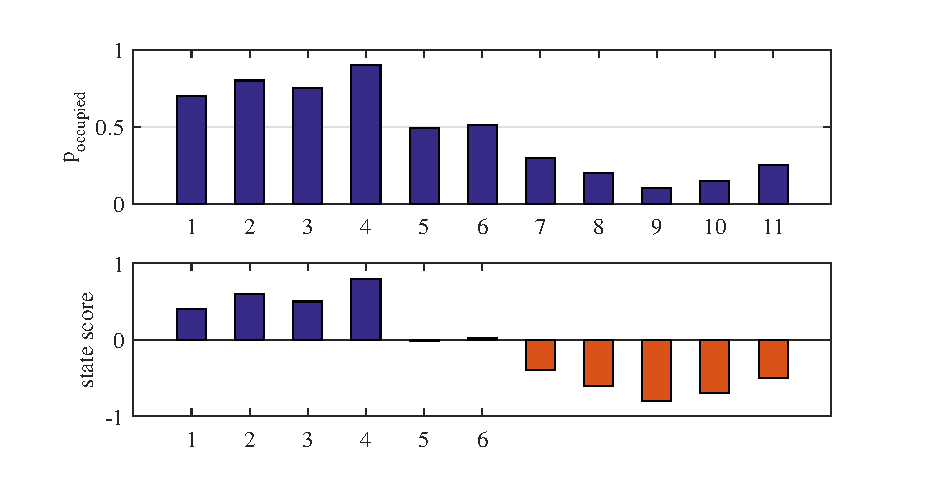
\includegraphics[scale=1]{chapters/mapping_of_dynamic_areas/figures/pmac_noise_problem_case}
\caption{}
\label{fig:pmac_noise_problem_case}
\end{figure}

\begin{figure}[htbp]
    \centering
    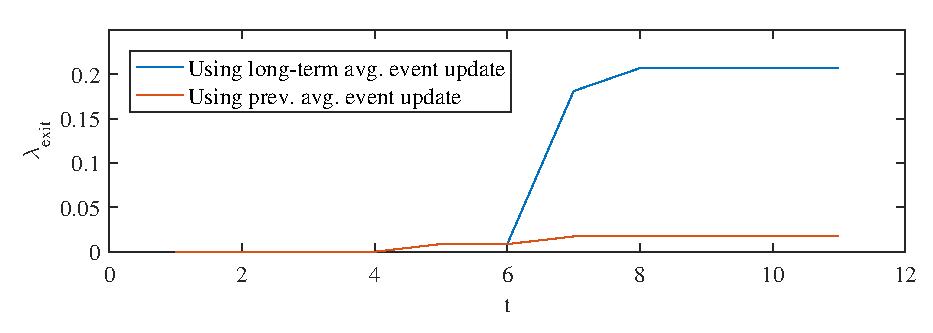
\includegraphics[scale=1]{chapters/mapping_of_dynamic_areas/figures/visualization_of_advantage_long_term_average}
    \caption{}
    \label{fig:visualization_of_advantage_long_term_average}
\end{figure}